\graphicspath{{../03Mathematics/pics/}}

\chapter{Mathematics}\label{ch:Mathematics}

\lettrine[lines=2]{\color{darkocre}I}{n} the previous chapter we
learned about numbers and various relations between them. As a
particular class of relations we discussed functions. We introduced
\emph{binary} and \emph{unary} functions and different ways
functions can be combined (\emph{composed}) to produce new
functions. We also learned
that functions can be
represented in various ways and that none of those different
representations defines
the concept of function completely. Each representation of a function
highlighted some important aspect of it.

\begin{myprereq}{Prerequisite Knowledge}
	To fully understand the material of this chapter, readers should be comfortable with the following concepts:
	
	\begin{itemize}
		\item \phantom{phantom}
		\vspace{-0.5cm}
		\item State
		\item Dynamical equations
	\end{itemize}	
\end{myprereq}


\section{Arrows}

To arrive at the idea of vectors we will start with simple geometrical
objects -- arrows in a plane, as illustrated in the Figure \ref{fig:arrowsSpace}.

\begin{SCfigure}%[htbp]
  %\centering
  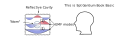
\includegraphics[scale=1.0]{defaultFigureTemplate}
  \caption{Set of arrows starting at the same origin point $O$. All
    imaginable arrows taken as one set form the arrow space
    $\overset{\Rightarrow}{A}$.}
  \label{fig:arrowsSpace}
\end{SCfigure}

Symbolically, we will denote vectors by placing an arrow over letters:
\[
\vec{a}\,,\vec{b}\,,\vec{c}\,,\ldots\,,\vec{\alpha}\,,\vec{\beta}\,.
\]

\subsection{Dirac Notation}

\section{Scalar Product}

To arrive at the idea of vectors we will start with simple geometrical
objects -- arrows in a plane, as illustrated in the Figure \ref{fig:arrowsSpace}.

\section{Operators}

To arrive at the idea of vectors we will start with simple geometrical
objects -- arrows in a plane.
\[
\braket{\phi}{\phi}
\]
and
\[
\ketbra{\phi}{\phi}\,.
\]

\subsection{Super-operators}

\section{Functionals}
Another important type of function is called \emph{functional}. A functional maps a function into a number. Let's consider several examples.

\subsection*{Total Mass}
Suppose an astrophysicist is trying to model a spherically symmetric star and calculates \emph{density} of the star as the function of distance from its center: $r\rightarrow\rho_r$. The total mass of the star can then be evaluated as the sum of masses of all spherical shells with thickness $\delta r$:
\[
M = \int \delta V\rho_r=\int 4\pi r^2\delta r\rho_r\,.
\]
For a given function $\rho_r$ this summation will result in a number -- star's total mass. Such mapping $\rho_r\rightarrow M$ is an example of a functional.

\subsection*{Total Fuel}
Consider a car moving on a straight highway between two points $A$ and $B$. The amount of fuel the engine consumes at a given moment depends on the speed of the car at that moment and can be described by the function $\mu_v$. Suppose the position of the car as the function of time $x_t$ is known and are looking for the total fuel consumed during the travel. This can be done in three steps. 

First, we find the speed of the car as the function of time by applying the operator $\partial_t$ to $x_t$: $v_t=\partial_{t}x$. Second, we find the fuel consuption rate $\mu$  as the function of time by plugging $v_t$ into $\mu_v$: $f_t = \mu(v_t)$. Finally, we can find the total amount of consumed fuel as the sum
\[
F = \int f_t\delta t\,.
\]
Combining all three steps into a single mathematical expression will result in a more cumbersome formula:
\[
F = \int \delta t\mu(\partial_t x)\,.
\]
This formula encodes a recipe for mapping any function $x_t$ into a number $F$ -- an example of a functional.

\subsection*{Total Action}
A body in a "freely fall" is moving with constant acceleration due to the force of gravity. Its speed increases as the body approaches the ground. If the body starts at rest at height $H$, its position along the vertical $y$ axis depends on time as $y_t=H-gt^2/2$ and the velocity changes according to the equation $v=-gt$.

The potenital energy $E_p=mgy$ of the body decreases, while its kinetic energy $E_k=mv^2/2$ grows. The total mechanical energy $E=E_p+E_k$ remains fixed according to the law of energy conservation. Thus, the potential energy of the body is transformed into the kinetic energy.

Another physical quantity is often important -- the \emph{imbalance} of kinetic energy over the potential energy:
\[
L = E_k - E_p\,.
\]
It does not remain constant, and for the case of a free fall we can easily find its time dependence:
\[
L_t = mg^2t^2 - mgH\,.
\]
Given $L_t$, we can calculate a fundamental physical quantity -- total \emph{action} of the process:
\[
A = \int\delta t L_t\,.
\]
The summation extends to the moment $t=T$ when the body reaches the ground ($y=0$). This happens at $T=\sqrt{2H/g}$.

Performing the summation requires evaluation of two familiar sums:
\[
\int t^2\delta t =\frac{T^3}{3}\quad\textrm{ and }\quad \int \delta t=T\,.
\]
Substituting the values of $T$ and simplifying, the expression for the total action takes the form
\[
A = mgT(\frac{gT^2}{3}-H)=-\frac{mH}{3}\sqrt{2gH}=-\frac{mv_{m}H}{3}\,.
\]
Here we used $v_m=gT=\sqrt{2Hg}$ -- the maximal speed of the body at the end of the free fall process. Finally, denoting the maximum momentum of the body as $p_m=mv_m$, we obtain $A=-p_m H/3$. Note that the action can be expressed as the product of momentum and distance.

\emph{Action} is a physical quantit of fundamental importance. It plays a prominent role in both classical mechanics (the principle of \emph{stationary action}) and in quantum physics (the principle of \emph{action quantization}). Both principles will be explored in details later in the book.

\begin{exercise}
	Calculate the total action of a free fall process for an electron falling from the height 0.1 meter.
\end{exercise}



\subsection*{Assorted Examples}
Examples of functionals given above involve evaluation of sums to find  total quantities of various kinds. 

\section{Spaces}

To arrive at the idea of vectors we will start with simple geometrical
objects -- arrows in a plane.
\[
\braket{\phi}{\phi}
\]
and
\[
\ketbra{\phi}{\phi}\,.
\]

\section{Application: Circular Motion}
Let us examine how the concepts and tools discussed above can be applied to a simple case of circular motion.  

Consider a  particle moving in a circle with the radius $R$, as shown in Figure X. If we choose the center of the circle as the reference point, we can specify the position of the particle using an arrow $\ket{r}$. During motion the direction of this arrow is constantly changing, but its length $R$ remains the same.  

After a short time interval $\delta t$, the position of the particle changes by $\delta\ket{r}$:
\[
\ket{r_t}\quad\rightarrow\quad \ket{r_{t+\delta t}} = \ket{r_t}+\delta\ket{r}\,.
\]

The length of the path covered by the particle during the time interval $\delta t$ can be approximated by the length of the arc  $\delta L=R\delta\theta=v\delta t$. The arrow $\delta\ket{r}$ can be written as $\delta L\ket{u}$ where $\ket{u}$ is the vector of unit length pointing in the direction of motion. This unit vector can be constructed from $\ket{r}$ by scaling it down by $R$ and then rotating counter-clockwise with the operator $\op{J}$: 
\[
\delta\ket{r}=R\delta\theta\op{J}\left(\frac{\ket{r}}{R}\right)\,.
\]
Since $\op{J}$ is a linear operator, the $R$ cancels and we can write
\[
\frac{\delta\ket{r}}{\delta t}=\frac{\delta\theta}{\delta t}\op{J}\ket{r}\qquad\Longrightarrow\qquad
\partial_t\ket{r}=\omega\op{J}\ket{r}\,,
\]
where we introduced the angular speed $\omega=\partial_t\theta$. Finally, by applying the $\op{J}$ operator to both sides of the last equation, we can cast it into the "Schrodinger" form:
\[
\op{J}\partial_t\ket{r}=-\omega\ket{r}\,.
\]  



\section*{Chapter Highlights}
{\setstretch{1.5}\chhc
  \it
\begin{itemize}
\item Arrows in a plane provide a simple model for vectors.
\item Arrows can be manipulated in ways analogous to numbers: Two arrows
  be added, an arrow can be ``scaled'' (stretched or compressed). Arrows form
  an algebra.
\item Basis is an extremely important concept. Basis is a set of
  objects (arrows) that can be used to ``build'' all other similar
  objects (arrows). At the same time, basis can not be used to build
  itself -- basis arrows are independent.
\end{itemize}
}
